%%%%%%%%%%%%%%%%%%%%%%%%%%%%%%%%%%%%%%%%%%%%%%%%%%%%%%%%%%%%%%%%%%%%%%%%%%%%%%%%
%% 
\cleardoubleoddpage%  Make sure to start each chapter on a new odd page
\chapter{Example}
\label{sec:example}


\section{How to Start?}
This is an example for another chapter in your thesis.
It should primarily show you some basic \LaTeX\ tricks.
For instance, \autoref{sec:introduction:motivation} references to your motivation.
You can also embed figures, tables, etc.\ in your work.
\autoref{fig:learningcenter} is an example for a figure (i.e.\ photos, diagrams, and other artwork).
Note that figures (just like tables, see \autoref{tab:nicetable}) are floating elements.
They are either placed at the top or bottom of a page (or sometimes stand on their own page), but not in between your text.
You can influence their placement with the placement modifiers ``t'', ``b'', and ``p''.
Bottom placement (``b'') is sometimes more tricky, as \LaTeX\ does not consider this nice in some situations.
You can convince \LaTeX\ to honor your placement expectation with ``!b'' then.
Please be aware that you typically do not want to place a float at the top of a chapter title page.
Since you do not place figures/tables in between your running text, you always need to reference them by their label (e.g.\ \autoref{fig:learningcenter} or \autoref{tab:nicetable}).
\begin{figure}[t]
\centering
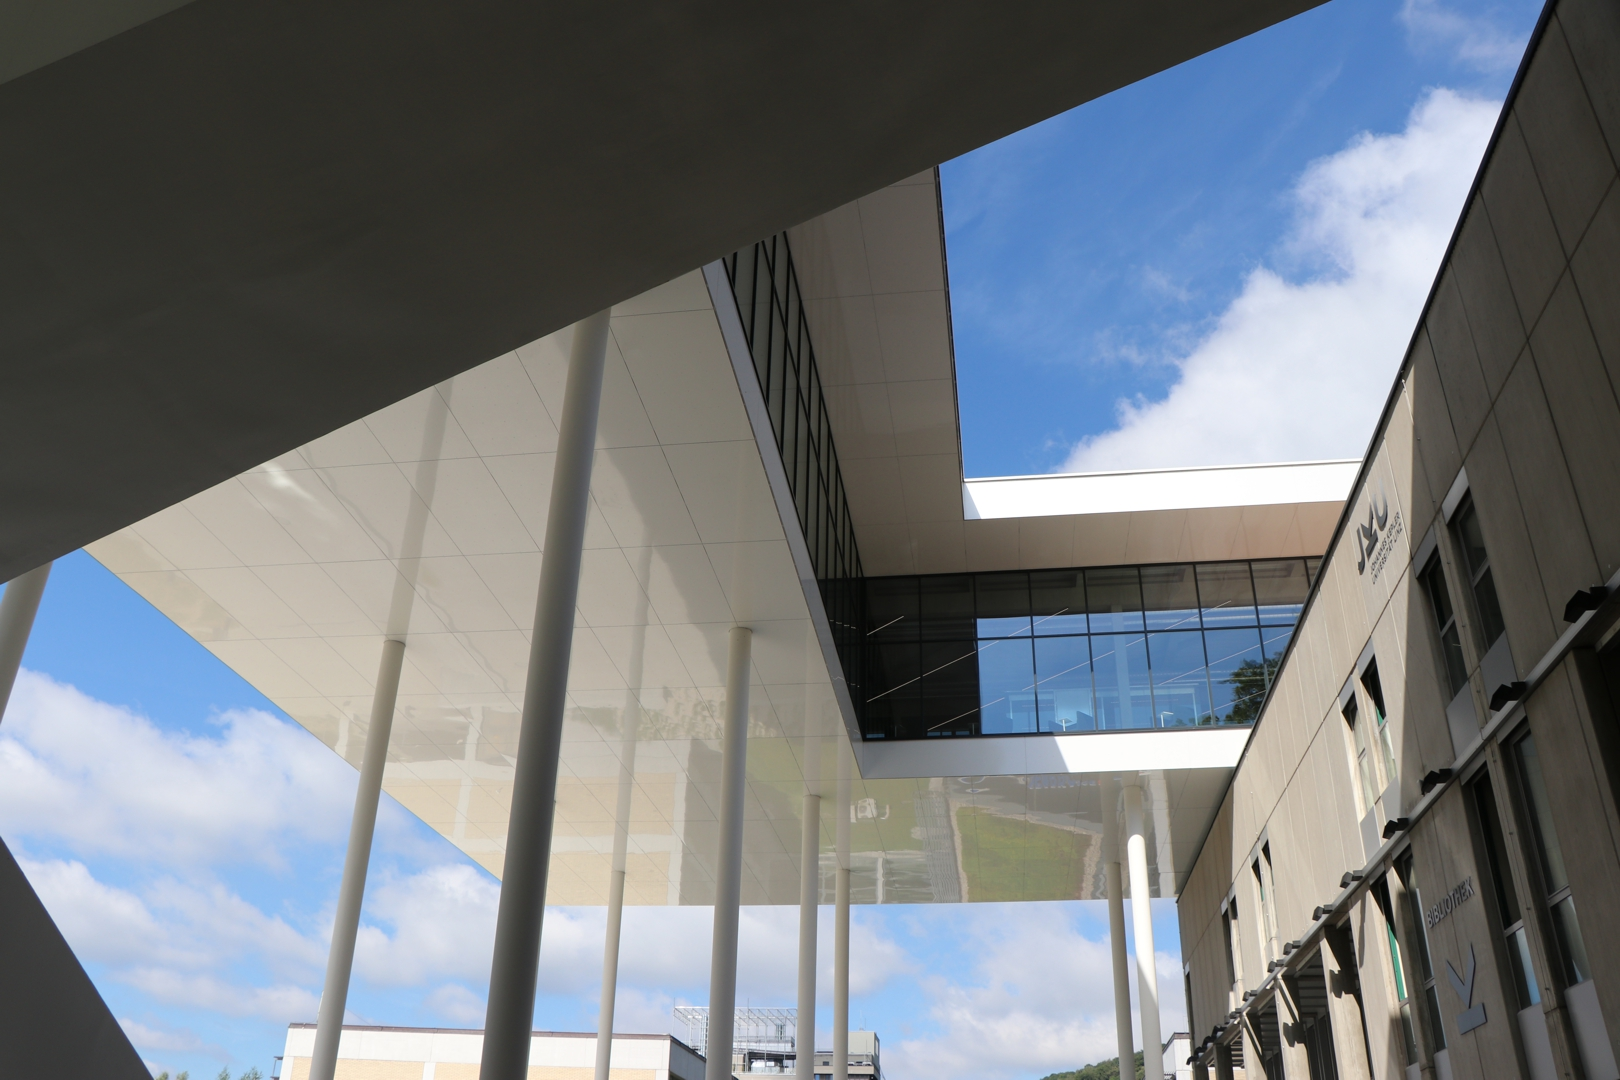
\includegraphics[width=\linewidth]{images/jku_learningcenter}
\caption{
    A figure. Be aware that figures have their caption below the artwork
}\label{fig:learningcenter}
\end{figure}
\begin{table}[b]
\centering
\caption{
    A table. Be aware that tables have their caption above the table
}\label{tab:nicetable}
\begin{tabularx}{\linewidth}{l>{\raggedright\arraybackslash}X}
\toprule
\textbf{Option}        & \textbf{Description} \\
\midrule
\texttt{phdthesis}     & PhD thesis \\
\texttt{mathesis}      & Master's thesis \\
\texttt{diplomathesis} & Diploma thesis \\
\texttt{bathesis}      & Bachelor's thesis \\
\texttt{seminarreport} & Seminar report \\
\texttt{techreport}    & Technical report \\
\bottomrule
\end{tabularx}
\end{table}

You will often reference and quote other works.
The source of these citations needs to be marked with the \string\cite\{\}\ command.
There are different ways to cite the work of others.
These are a few examples:
\begin{itemize}
\item The Tor directory authority moria1 shows a voting behavior for the HSDir flag that significantly deviates from that of other directory authorities~\cite{bib:2021-hoeller-iiwas}. Be aware that the \string\cite\ command is part of the sentence and, hence, comes before the period.
\item Roland~\cite{bib:2015-roland-thesis-book} proposes a novel attack concept against NFC secure elements in mobile phones.
\item Roland and Langer~\cite{bib:2013-roland-woot} uncovered a flaw in legacy-support of the MasterCard contactless payment protocols that allows an attacker to clone certain credit cards.
\item Höller et al.~\cite{bib:2021-hoeller-foci} designed an experiment to measure the usage of Tor V3 onion services in a privacy-conscious way. Here we used ``et al.'' because the cited work has more than two authors.
\item Höller et al.~\cite{bib:2021-hoeller-iiwas} conclude:
\begin{quote}
\emph{Ultimately, the high fluctuations in the hidden service directory were caused by a mixture of several issues. First the changed voting behavior of three directory authorities reduced the amount of obtainable votes to six. If any of the remaining six relays went offline -- which tends to happen during ongoing DOS attacks -- relays needed to obtain five out of five available votes. So any individual measurement failure regarding either bandwidth or uptime led to a withdrawn HSDir flag.}
\end{quote}
\item You sometimes also paraphrase from multiple sources. For that purpose, the \string\cite\ command accepts a list of multiple comma-separated references. Do not add spaces inbetween them. Various analyses of the Tor network have been performed recently~\cite{bib:2021-hoeller-foci,bib:2021-hoeller-iiwas}. 
\end{itemize}

%% 
%%%%%%%%%%%%%%%%%%%%%%%%%%%%%%%%%%%%%%%%%%%%%%%%%%%%%%%%%%%%%%%%%%%%%%%%%%%%%%%%
